%Solución del Ejercicio 3 por medio de la metodología 6D

\subsection{Descripción del problema}
Dada una circunferencia con centro en el punto $C$ con coordenadas $(x_{1}, y_{1})$ y radio $r$, evaluar si un punto $T$ con coordenadas $(x_{2}, y_{2})$ esta dentro del área de la circunferencia.\\
\subsection{Definición de la solución}
La circunferencia es un punto que está a una misma distancia de un punto fijo llamado centro. 
La distancia de cada punto de la circunferencia al centro se llama radio.
\begin{equation}
    (x-h)^2 + (y-k)^2 =r^2
\end{equation}
\subsection{Diseño de la solución}
Para resolver estas ecuaciones y determinar si un punto T con coordenadas $(x_{2}, y_{2})$ esta dentro del área de la circunferencia con centro en el punto $C$ el cual utiliza coordenadas $(x_{1}, y_{1})$ y radio, se calcula la distancia del punto T y el centro de la circunferencia utilizando la formula de la distancia entre dos puntos $(x_{1}, y_{1})$ y $(x_{2}, y_{2})$.\\
\begin{equation}
 d = \sqrt{{(x_2 - x_1)^2 + (y_2 - y_1)^2}} 
\end{equation}
\begin {figure}[h!]
\centerline{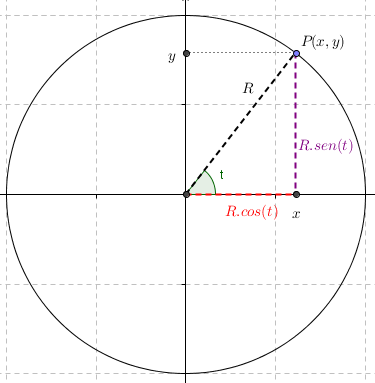
\includegraphics[width = 6cm]{Latex-imágenes/fig3.png}}
\caption{Gráfica de la ecuación.}
\label{fig}
\end {figure}
\begin{enumerate}
    \item Si $d <= r$, el punto T esta dentro del área de la circunferencia.\\
    \item Si $d > r$, el punto T esta fuera del área de la circunferencia.\\
\end{enumerate}
Se realizo un diagrama de flujo para saber como solucionar el problema.\\
\begin {figure}[h!]
\centerline{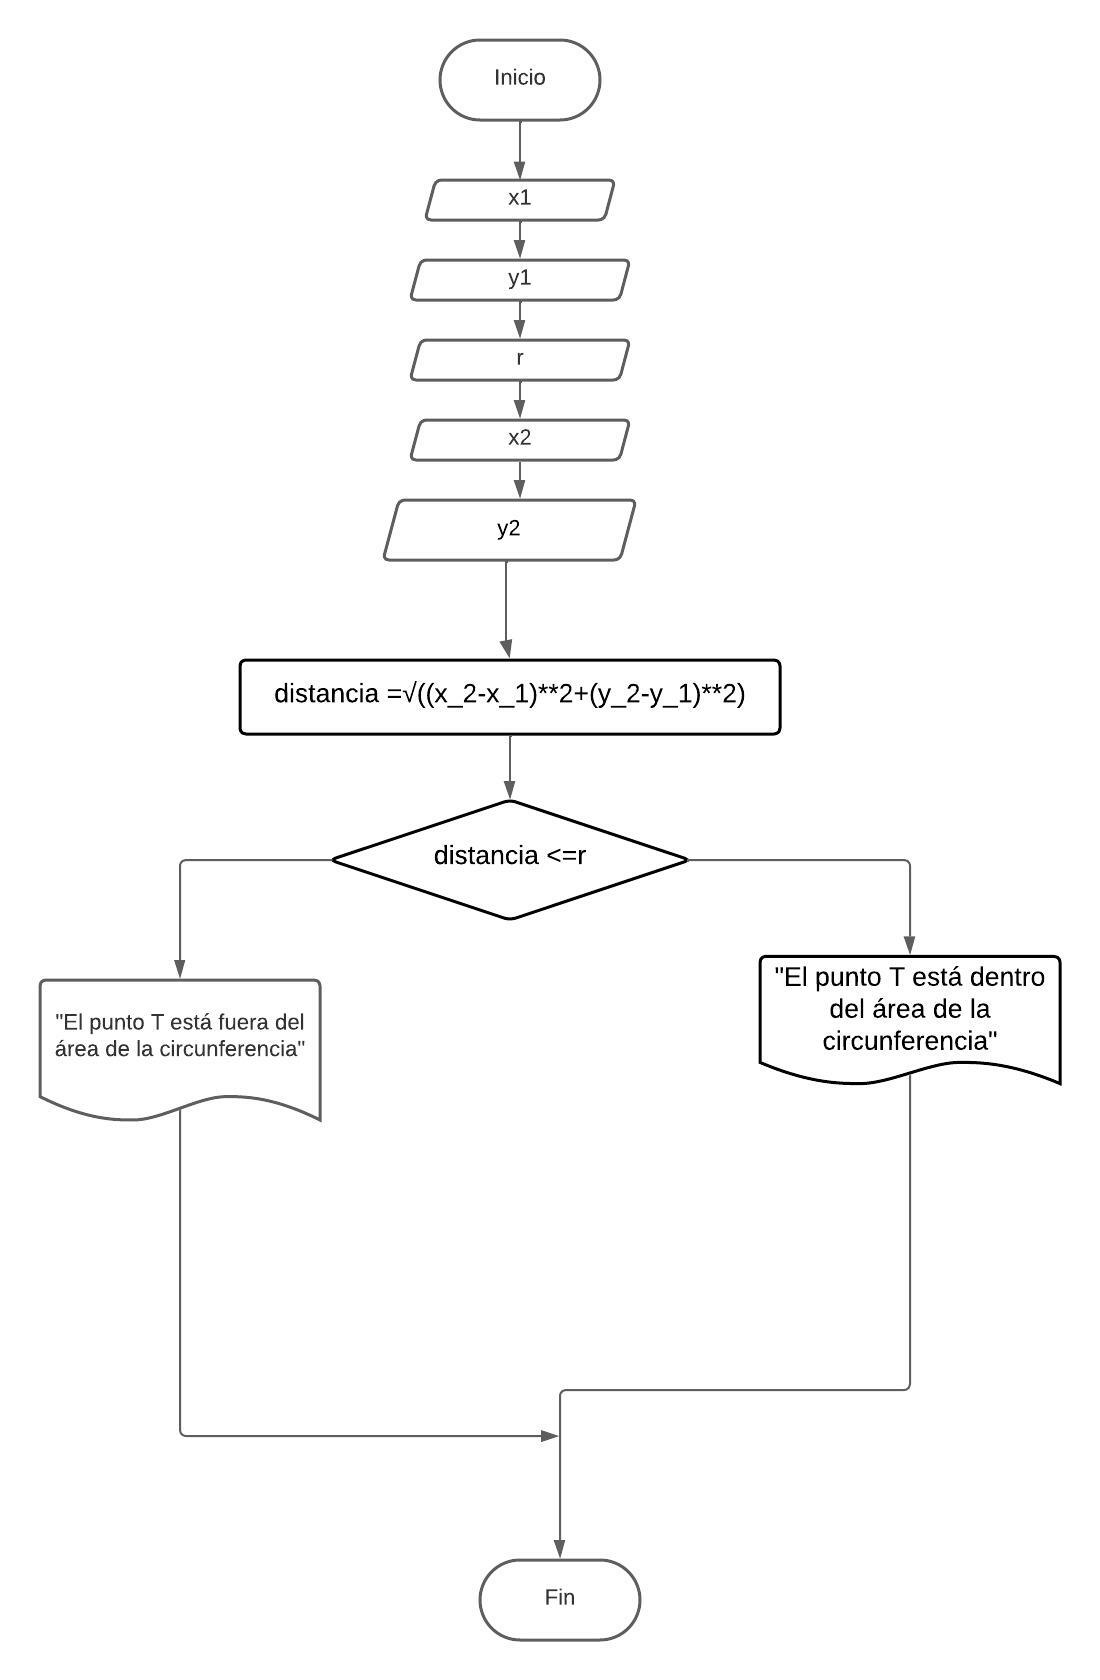
\includegraphics[width = 6cm]{Latex-imágenes/Diagrama de la circunferencia .jpeg}}
\caption{Diagrama de flujo de la solución}
\label{fig}
\end {figure}
\subsection{Desarrollo de la solución}
Para este problema se implemento este código en Apache NetBeans 14 con lenguaje en Java, donde al principio del bloque pide al usuario que ingrese las variables de la ecuación de la distancia entre dos puntos, las cuales son: $x_{1},y_{1},r,x_{2},y_{2}$
\begin{javaCode}
  double x1 = Double.parseDouble(JOptionPane.showInputDialog
       ("Ingrese la coordenada x1:"));
  double y1 = Double.parseDouble(JOptionPane.showInputDialog
       ("Ingrese la coordenada y1:"));
  double r = Double.parseDouble(JOptionPane.showInputDialog
       ("Ingrese el radio r de la circunferencia:"));
  double x2 = Double.parseDouble(JOptionPane.showInputDialog
       ("Ingrese la coordenada x2 del punto T:"));
  double y2 = Double.parseDouble(JOptionPane.showInputDialog
       ("Ingrese la coordenada y2 del punto T:"));
\end{javaCode}
Después se programo el proceso del código  el cual es la ecuación de la distancia.
\begin{javaCode}
    double distancia = Math.sqrt(Math.pow(x2 - x1, 2) + Math.pow(y2 - y1, 2));
\end{javaCode}
En el bloque final del código se presenta una condición, si la distancia es menor o igual al radio entonces el punto T está dentro del área de la circunferencia y si, no el punto T está fuera del área de la circunferencia.
\begin{javaCode}
 if (distancia <= r) {
            // Salida
            JOptionPane.showMessageDialog(null, "El punto T está dentro del área de la circunferencia.");
        } else {
            JOptionPane.showMessageDialog(null, "El punto T está fuera del área de la circunferencia.");
        }
\end{javaCode}
\subsection{Depuración y pruebas}
\begin{table}[!ht]
\label{T:equipos}
\begin{center}
\begin{tabular}{| c | c | c | c | c | c |}
\hline
\textbf{$x_{1}$} & \textbf{$y_{1}$} & \textbf{$r_x$} & \textbf{$x_{2}$} & \textbf{$y_{2}$} & \textbf{Fuera o Dentro}\\
\hline
0 & 0 & 2 & 4 & 4 & Fuera \\
0 & 1 & 2 & 3 & 4 & Fuera \\
7 & 7 & 8 & 6 & 6 & Dentro \\
20 & 10 & 9 & 5 & 5 & Fuera\\
0 & 0 & 3 & 1 & 1 & Dentro\\
\hline
\end{tabular}
\caption{Tabla de corridas.}
\end{center}
\end{table}
